\chapter{Introduction to the Template}

\section{The purpose of this package}
This template provides a streamlined design for typesetting books. Welcome to feedback bugs or ideas via email \href{mailto:xiamyphys@gmail.com}{\ttfamily xiamyphys@gmail.com} or \href{https://github.com/xiamyphys/litebook}{GitHub}.

This template is used by me to reformat the textbook \href{https://github.com/xiamyphys/LaTeX-General-Relativity-R.Wald}{\emph{General Relativity, R. Wald}}, and I also use this template to typesetting my notes on \href{https://github.com/xiamyphys/Group-Theory-in-Physics}{\emph{Group Theory in Physics}}. You can download them on \href{https://github.com/xiamyphys}{GitHub}.

\section{Installing \pkg{LiteBook} and loading it}
For portable version, simply download latest \verb|litebook.cls| file from \href{https://github.com/xiamyphys/LiteBook}{GitHub} or \href{https://ctan.org/pkg/litebook}{CTAN} and save it under your working directory. This way of installation is simple and convenient, but you have to manually update \verb|.cls| now and then.

However, I strongly suggest that you should use terminal/cmd to implement the commands to update all the packages (and install this package) to the latest version or switch to portable version instead
\begin{verbatim}
    sudo tlmgr update --self --all
\end{verbatim}

If you are in some areas with awful Internet environment (such as GFW), you can choose a proper mirror source or use other means\footnote{Please comply with local network regulations.}. To learn more, please refer to \href{https://tex.stackexchange.com/questions/55437/how-do-i-update-my-tex-distribution}{How do I update my \hologo{TeX} distribution?}

\section{Compatibility}
The test environments are macOS + Mac\hologo{TeX} 2024 / Overleaf / Ubuntu 22.04.2 and they all work fine for \hologo{pdfLaTeX} and \hologo{XeLaTeX} compilers. Windows and Unix platforms' unknown. The compiling time of current document via \hologo{pdfLaTeX} compiler is about \verb|1s| on \textsf{MacBook Air M2 8 GB (macOS 14.4.1)} when charging.

\section{Cover configurations}
There are several lines of information and a cover image on the cover of this document, the corresponding commands are the following

\begin{verbatim}
    \cover{\UPLOWFadingImage[trim={0 {.9\paperheight} 0 0},clip]{cover}
                            [trim={0 {.5\paperheight} 0 0},clip]{cover}}
    \title{\scshape The \pkg{LiteBook} Template}
    \subtitle{Version 0.2b \today}        \author{Hsia Mingyu}
    \bioinfo{Hangzhou Dianzi University}
    \press{\scshape The University of Chicago Press}
\end{verbatim}

The same as the \pkg{book} class, the macro \cmd{title} could not be omitted, or it will return an error, and there will be a warning if the macro \cmd{author} is omitted. The \cmd{cover} can assign the format of the image on the cover and you can adjust the format of the image with the \pkg{fadingimage} package.

\section{Math options of this template}
\begin{verbatim}
    \documentclass[<math>]{litebook}
\end{verbatim}

You can set the math font to be \mode{newtx} (default) or \mode{mtpro2}.

\section{Preset packages and commands}
This template has preset with the following packages:
\begin{table}[!ht]
    \centering
    \begin{tabular}{l l l l l l l l}
        \toprule
        \pkg{amsthm} & \pkg{bm} & \pkg{cancel} & \pkg{derivative} & \pkg{esvect} & \pkg{extarrows} & \pkg{fixdif} & \pkg{nicefrac}\\
        \midrule
        \pkg{nicematrix} & \pkg{physics2} & \pkg{refstyle} & \pkg{siunitx} & \pkg{booktabs} & \pkg{diagbox} & \pkg{fontawesome5} & \pkg{geometry}\\
        \midrule
        \pkg{indentfirst} & \pkg{mdframed} & \pkg{multicol} & \pkg{multirow} & \pkg{setspace} & \pkg{tabularx} & \pkg{tikz} & \pkg{xcolor}\\
        \bottomrule
    \end{tabular}
\end{table}

You can click on them to go to the homepage to view the documentation.

And commands \verb|\i|, \verb|\e|, \verb|\T| have been defined to input 
$\i$, $\e$ in roman (non-italic) text and matrix transpose symbol $\T$, which can help you typeset math quickly.

The template has preset the following commands for different type of references via \pkg{refstyle} package: \verb|\eqref{<label>}|, \verb|\figref{<label>}| and \verb|\tabref{<label>}|, you can add other ref commands via \pkg{refstyle} package.

\section{Equation test}
The following is the Schr\"odinger Equation
\begin{equation}
    \i\hbar\pdv{}t\Psi(\bm r,t)=\ab[-\frac{\hbar^2}{2m}\nabla^2+V(\bm r,t)]\Psi(\bm r,t)
    \label{1.7.1}
\end{equation}

\Eqref{1.7.1} is the time-dependent Schr\"odinger Equation for the nonrelativistic particle.

\section{Figure and caption side by side test}
\begin{figure}[htbp]
\begin{minipage}{.32\textwidth}
    \caption{A diagram showing the causal structure of spacetime in special relativity. The ``light cone'' of $p$ rather than a ``surface of simultaneity'' with $p$ now plays a fundamental role in determining the causal relationship of $p$ to other events.}
    \label{1.1}
\end{minipage}
\hfill
\begin{minipage}{.64\textwidth}
    \centering
    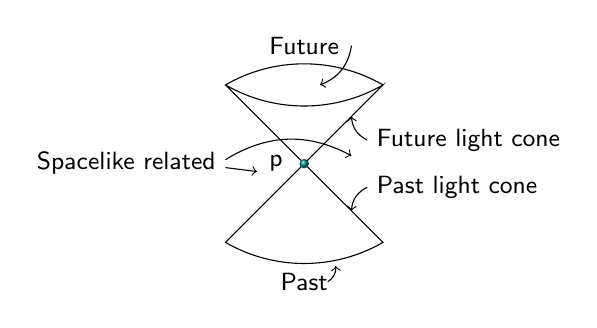
\begin{tikzpicture}
        \draw (-1,1) -- (1,-1) arc (-60:-120:2) -- (1,1) arc (-60:-120:2) arc (-60:-120:-2);
        \shade [ball color=teal] (0,0) circle (.06) node [anchor=east,xshift=-1ex] {\sffamily\small p};
        \node at (0,1.5) {\sffamily\small Future};
        \path [->] (.6,1.5) edge [bend left] (.2,1);
        \node at (0,-1.5) {\sffamily\small Past};
        \path [->] (.3,-1.5) edge [bend right] (.4,-1.3);
        \node [left] at (-1,0) {\sffamily\small Spacelike related};
        \path [->] (-1,-.05) edge (-.6,-.1);
        \path [->] (-1,.05) edge [bend left] (.6,.1);
        \node [right] at (.8,.3) {\sffamily\small Future light cone};
        \path [->] (.8,.3) edge [bend left] (.6,.6);
        \node [right] at (.8,-.3) {\sffamily\small Past light cone};
        \path [->] (.8,-.3) edge [bend right] (.6,-.6);
    \end{tikzpicture}
\end{minipage}
\end{figure}

Here, \figref{1.1} is a diagram showing the causal structure of spacetime in special relativity.